\chapter{cursors}
\label{sec:cursors}
\lhead[tempest]{}
\lstset{style=6502Style}
The Tempest source code refers to the player's ship as a \icode{CURSOR}. It does this because it
is the 1980s and that is what you call something on the screen that you can control.

The graphics in Tempest are generated using Atari's 'Quadrascan' vector
technology. The images are all defined using a series of vectors. A vector in
this case is a (X,Y) value pair that moves the beam in an X,Y direction to a
new point on the screen. A series of vectors moving from point to point around
the screen will eventually form a complete image.

When we take a look at the data structure defining a relatively upright version of the
player's ship we find this. I'm going to speculate that \icode{NCSR4S} is short
for 'New Cursor 4 Start' and \icode{NCSR4E} for 'New Cursor 4 End':
\begin{lstlisting}
NCRS4S:
        VEC 3,-2
        VEC 5,2
        VEC -3,1
        VEC 2,-1
        VEC -4,-1
        VEC -2,1
        VEC 2,1
        VEC -3,-1
NCRS4E:
\end{lstlisting}

The number pairs in the above listing are the vectors we're talking about, and we're going to see how we can use them to build up
an image of the ship assuming an origin point of zero. Our first step, therefore,
is to draw a line from (0,0) to (3,-2) as follows:

\begin{figure}[H]
    \centering
    \begin{adjustbox}{width=7cm,center}
      \includegraphics[width=12cm]{src/cursors/build_cursor_2_3.png}%
    \end{adjustbox}
  \caption{Draw a line from \icode{(0,0)} to \icode{(3,-2)}.}
\end{figure}

Our next step reveals a bit more about the actual nature of the operation we are performing. To
draw a line from our new position using a vector of \icode{5,2} we add it to our current
position of \icode{(3,-2)} to draw a line to \icode{8,0}:
\begin{figure}[H]
  \centering
  \begin{adjustbox}{width=7cm,center}
    \includegraphics[width=12cm]{src/cursors/build_cursor_3_6.png}%
  \end{adjustbox}
  \caption{\icode{(3,-2)} + 
         \icode{(5,2)}.
          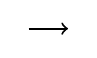
\begin{tikzpicture}
            \draw[->,line width=0.7pt] (0,0) to (0.5,0);
          \end{tikzpicture}
         \icode{(8,0)}
         }
\end{figure}

With this as our method, we can start building up our complete image, adding each vector in
our array to the previous result to define a new line to draw.

\begin{figure}[H]
  {
    \setlength{\tabcolsep}{3.0pt}
    \setlength\cmidrulewidth{\heavyrulewidth} % Make cmidrule = 
    \begin{adjustbox}{width=15cm,center}
      \begin{subfigure}{0.3\textwidth}
        \begin{figure}[H]
          \centering
          \begin{adjustbox}{width=3cm,center}
            \includegraphics[width=12cm]{src/cursors/build_cursor_4_6.png}%
          \end{adjustbox}
          \caption{\icode{(8,0)} + 
                 \icode{(-3,1)}.
                  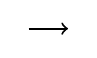
\begin{tikzpicture}
                    \draw[->,line width=0.7pt] (0,0) to (0.5,0);
                  \end{tikzpicture}
                 \icode{(5,1)}
                 }
        \end{figure}
      \end{subfigure}
      \begin{subfigure}{0.3\textwidth}
        \begin{figure}[H]
          \centering
          \begin{adjustbox}{width=3cm,center}
            \includegraphics[width=12cm]{src/cursors/build_cursor_5_6.png}%
          \end{adjustbox}
          \caption{\icode{(5,1)} + 
                 \icode{(2,-1)}.
                  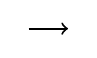
\begin{tikzpicture}
                    \draw[->,line width=0.7pt] (0,0) to (0.5,0);
                  \end{tikzpicture}
                 \icode{(7,0)}
                 }
        \end{figure}
      \end{subfigure}
      \begin{subfigure}{0.3\textwidth}
        \begin{figure}[H]
          \centering
          \begin{adjustbox}{width=3cm,center}
            \includegraphics[width=12cm]{src/cursors/build_cursor_6_6.png}%
          \end{adjustbox}
          \caption{\icode{(7,0)} + 
                 \icode{(-4,-1)}.
                  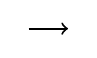
\begin{tikzpicture}
                    \draw[->,line width=0.7pt] (0,0) to (0.5,0);
                  \end{tikzpicture}
                 \icode{(3,-1)}
                 }
        \end{figure}
      \end{subfigure}
    \end{adjustbox}
    }\caption[]{Starting to take shape.}
\end{figure}

Adding our last three vectors completes the picture, and we have a claw.
\begin{figure}[H]
  {
    \setlength{\tabcolsep}{3.0pt}
    \setlength\cmidrulewidth{\heavyrulewidth} % Make cmidrule = 
    \begin{adjustbox}{width=15cm,center}
      \begin{subfigure}{0.3\textwidth}
        \begin{figure}[H]
          \centering
          \begin{adjustbox}{width=3cm,center}
            \includegraphics[width=12cm]{src/cursors/build_cursor_7_6.png}%
          \end{adjustbox}
          \caption{\icode{(3,-1)} + 
                 \icode{(-2,1)}.
                  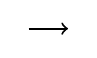
\begin{tikzpicture}
                    \draw[->,line width=0.7pt] (0,0) to (0.5,0);
                  \end{tikzpicture}
                 \icode{(1,0)}
                 }
        \end{figure}
      \end{subfigure}
      \begin{subfigure}{0.3\textwidth}
        \begin{figure}[H]
          \centering
          \begin{adjustbox}{width=3cm,center}
            \includegraphics[width=12cm]{src/cursors/build_cursor_8_6.png}%
          \end{adjustbox}
          \caption{\icode{(1,0)} + 
                 \icode{(2,1)}.
                  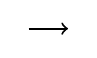
\begin{tikzpicture}
                    \draw[->,line width=0.7pt] (0,0) to (0.5,0);
                  \end{tikzpicture}
                 \icode{(3,1)}
                 }
        \end{figure}
      \end{subfigure}
      \begin{subfigure}{0.3\textwidth}
        \begin{figure}[H]
          \centering
          \begin{adjustbox}{width=3cm,center}
            \includegraphics[width=12cm]{src/cursors/build_cursor_9_6.png}%
          \end{adjustbox}
          \caption{\icode{(3,1)} + 
                 \icode{(-3,-1)}.
                  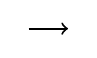
\begin{tikzpicture}
                    \draw[->,line width=0.7pt] (0,0) to (0.5,0);
                  \end{tikzpicture}
                 \icode{(0,0)}
                 }
        \end{figure}
      \end{subfigure}
    \end{adjustbox}
    }\caption[]{Putting the final pieces in place.}
\end{figure}

Finally, here are all of the \icode{CURSOR} elements along with their data structures.

\begin{minipage}[b]{0.48\linewidth}
\begin{figure}[H]
    \centering
    \begin{adjustbox}{width=4.5cm,center}
      \includegraphics[width=12cm]{src/cursors/final_cursor_0.png}%
    \end{adjustbox}
\end{figure}
\end{minipage}
\begin{minipage}[b]{0.48\linewidth}
\begin{lstlisting}
NCRS1S:
	VEC 0,-2
	VEC 2,-1
	VEC 3,4
	VEC -3,-3
	VEC -1,0
	VEC 0,2
	VEC 2,1
	VEC -3,-1
NCRS1E:
\end{lstlisting}
\end{minipage}

\begin{minipage}[b]{0.48\linewidth}
\begin{figure}[H]
    \centering
    \begin{adjustbox}{width=4.5cm,center}
      \includegraphics[width=12cm]{src/cursors/final_cursor_1.png}%
    \end{adjustbox}
\end{figure}
\end{minipage}
\begin{minipage}[b]{0.48\linewidth}
\begin{lstlisting}
NCRS2S:
	VEC 1,-2
	VEC 7,2
	VEC -3,1
	VEC 2,-1
	VEC -6,-1
	VEC 0,1
	VEC 2,1
	VEC -3,-1
NCRS2E:
\end{lstlisting}
\end{minipage}

\begin{minipage}[b]{0.48\linewidth}
\begin{figure}[H]
    \centering
    \begin{adjustbox}{width=4.5cm,center}
      \includegraphics[width=12cm]{src/cursors/final_cursor_2.png}%
    \end{adjustbox}
\end{figure}
\end{minipage}
\begin{minipage}[b]{0.48\linewidth}
\begin{lstlisting}
NCRS3S:
	VEC 2,-2
	VEC 6,2
	VEC -3,1
	VEC 2,-1
	VEC -5,-1
	VEC -1,1
	VEC 2,1
	VEC -3,-1
NCRS3E:
\end{lstlisting}
\end{minipage}

\begin{minipage}[b]{0.48\linewidth}
\begin{figure}[H]
    \centering
    \begin{adjustbox}{width=4.5cm,center}
      \includegraphics[width=12cm]{src/cursors/final_cursor_3.png}%
    \end{adjustbox}
\end{figure}
\end{minipage}
\begin{minipage}[b]{0.48\linewidth}
\begin{lstlisting}
NCRS4S:
	VEC 3,-2
	VEC 5,2
	VEC -3,1
	VEC 2,-1
	VEC -4,-1
	VEC -2,1
	VEC 2,1
	VEC -3,-1
NCRS4E:
\end{lstlisting}
\end{minipage}

\begin{minipage}[b]{0.48\linewidth}
\begin{figure}[H]
    \centering
    \begin{adjustbox}{width=4.5cm,center}
      \includegraphics[width=12cm]{src/cursors/final_cursor_4.png}%
    \end{adjustbox}
\end{figure}
\end{minipage}
\begin{minipage}[b]{0.48\linewidth}
\begin{lstlisting}
NCRS5S:
	VEC 5,-2
	VEC 3,2
	VEC -3,1
	VEC 2,-1
	VEC -2,-1
	VEC -4,1
	VEC 2,1
	VEC -3,-1
NCRS5E:
\end{lstlisting}
\end{minipage}

\begin{minipage}[b]{0.48\linewidth}
\begin{figure}[H]
    \centering
    \begin{adjustbox}{width=4.5cm,center}
      \includegraphics[width=12cm]{src/cursors/final_cursor_5.png}%
    \end{adjustbox}
\end{figure}
\end{minipage}
\begin{minipage}[b]{0.48\linewidth}
\begin{lstlisting}
NCRS6S:
	VEC 6,-2
	VEC 2,2
	VEC -3,1
	VEC 2,-1
	VEC -1,-1
	VEC -5,1
	VEC 2,1
	VEC -3,-1
NCRS6E:
\end{lstlisting}
\end{minipage}

\begin{minipage}[b]{0.48\linewidth}
\begin{figure}[H]
    \centering
    \begin{adjustbox}{width=4.5cm,center}
      \includegraphics[width=12cm]{src/cursors/final_cursor_6.png}%
    \end{adjustbox}
\end{figure}
\end{minipage}
\begin{minipage}[b]{0.48\linewidth}
\begin{lstlisting}
NCRS7S:
	VEC 7,-2
	VEC 1,2
	VEC -3,1
	VEC 2,-1
	VEC 0,-1
	VEC -6,1
	VEC 2,1
	VEC -3,-1
NCRS7E:
\end{lstlisting}
\end{minipage}

\begin{minipage}[b]{0.48\linewidth}
\begin{figure}[H]
    \centering
    \begin{adjustbox}{width=4.5cm,center}
      \includegraphics[width=12cm]{src/cursors/final_cursor_7.png}%
    \end{adjustbox}
\end{figure}
\end{minipage}
\begin{minipage}[b]{0.48\linewidth}
\begin{lstlisting}
NCRS8S:
	VEC 3,1,0
	VEC 3,-4
	VEC 2,1
	VEC 0,2
	VEC -3,1
	VEC 2,-1
	VEC 0,-2
	VEC -1,0
	VEC -3,3
NCRS8E:
\end{lstlisting}
\end{minipage}

